\section{Final Grade}
\label{gesamtnote}
Select a course under \url{https://cis.technikum-wien.at}-$>$ My CIS-$>$ My LV. Click the "`Final Grade"' symbol on the overview page to open the "`Final Grade"' page.

\subsection{Entering the Final Grade}
\subsubsection{Manually Entering the Final Grade }
\label{ben}

\begin{enumerate}
\item Enter the grade (1) and accept it with the '-$>$' - button.
\item After you have entered all the grades, you can then approve them (see chapter \ref{freigabe} on page \pageref{freigabe}\\).
\end{enumerate}

\begin{figure}[ht]
\begin{center}
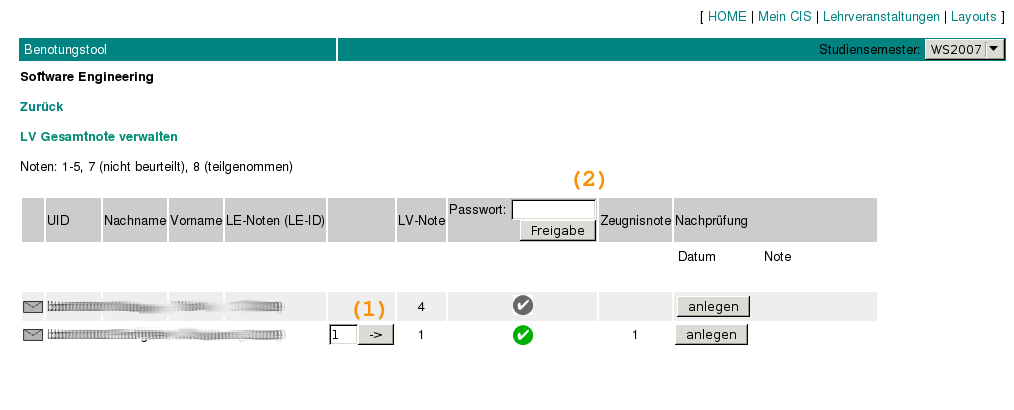
\includegraphics[width=1.0\textwidth]{benotungstool_benotung_lv.png}
\end{center}
\caption{Grading a Course}\label{benotung_lv}
\end{figure}

\subsubsection{Importing Grades from the Activity Tool (Checklist Tool)}
\label{ben}

If an activity has been created and graded in the activity tool (checklist tool) the grade will appear in the final grade.
If the course contains multiple teaching units, the average of all the grades will be suggested as the final grade.

The grade fields are already filled out. Click the '-$>$'- button to accept the grades.

\subsubsection{Importing Grades from Moodle}
\label{ben}

If a Moodle course has been created and graded, the grade will automatically appear in the final grade.
If the course contains multiple Moodle courses, the average of all the grades will be suggested as the final grade.
The grade fields are already filled out. Click the '-$>$'- button to accept the grades.

\subsubsection{Importing Grades from Excel}
\label{ben}

You can also import grades from an Excel file. To do so, use the following steps:

\begin{enumerate}
\item Download the Excel file with the grade list from CIS -$>$ Courses -$>$ Attendance and Grade Lists -$>$ Grade List.
\item Enter the grades in the Excel file.
\item Select the student number and grade columns in Excel for those students for whom you want to import the grades. (no heading)
\begin{figure}[ht]
\begin{center}
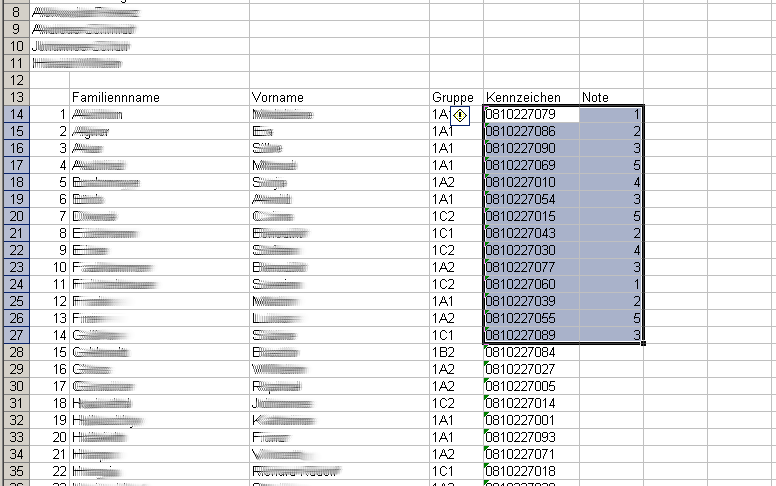
\includegraphics[width=1.0\textwidth]{CIS_Gesamtnote_Excelimport.png}
\end{center}
\caption{Importing from Excel}\label{excelimport}
\end{figure}
\item Copy the marked columns to the clipboard with $<$CTRL$>$+$ <$c$>$ or edit$ >$ copy.
\item Finally, click on the "`Import"' button to import the grades.
\end{enumerate}
\achtung {Existing grades are overwritten without a prompt.}
In order for the grade import to function properly, it is necessary to change some security settings for the browser:

\begin{enumerate}
\item Firefox / Mozilla
	\begin{enumerate}
	\item Open a new browser window.
	\item Enter "`about:config"' in the address bar. 
	(A warning message may appear, which you can skip by single clicking the displayed button)
	\item Search for the entry "`signed.applets.codebase\_principal\_support"'
	\item Change the setting to "`true"' by double clicking it.
	\end{enumerate}
	\achtung {Activating this setting creates a security hole. Therefore, we recommend disabling this setting again after you have finished importing the grades.}
\item InternetExplorer
	\begin{enumerate}
	\item It is not necessary to change any settings when using IE. When you click "Import" a warning message will appear (in IE7) that you will have to confirm by clicking on "`Allow access"'.
	\end{enumerate}
\item Safari, Opera
	\begin{enumerate}
	\item It is NOT POSSIBLE to import grades using the Safari or Opera web browser. Please use Firefox or Internet Explorer.
	\end{enumerate}
\end{enumerate}

\subsection{Approving Grades}
\label{freigabe}

Once you have entered all the grades you want to enter at this time (you can return to enter more grades at any time!) you can approve them for the administrative assistant with the "`Approve"' button (in the table header).
(2)

\info {NOTICE!! For reasons of increased security it is necessary to enter your password when approving grades.\footnote {This refers to your TW password which is used to log into the CIS webpage or the TW computers.}
}

\begin{itemize}
	\item Valid Grades: 1-5, 7 (not graded), 8 (participated)
	\item An information email is sent to you and the administrative assistant for the degree program when the grades are approved. The email includes the student number, first name, last name and grade for the new or edited entries.
	\item Approved entries are marked with a green circle with a check mark.
	\item If you change a grade that has already been approved, it will be marked with a grey circle with a check mark (as a notice for you that the administrative assistant has not yet been informed by email. However, they will still see the new grade immediately in their system interface.)
	\item The administrative assistant can import the approved grade as the transcript grade which will then appear in the next field for your verification.
	\item If the transcript grade differs from the grade you approved, the former is marked with a red border.
\end{itemize}

\subsection{Entering a Resit (2nd Date)}
\label{nachpruefung}

Once you have entered a final grade for a course, a button will appear (after refreshing the page by approving the grades for example) right next to the transcript grade for entering a resit. Once you have entered the resit, a date and grade as well as the "Edit" button will appear (see Fig.\ref{benotung_lv_nachpruefung_quick} (1),(2)).

\begin{figure}[ht]
\begin{center}
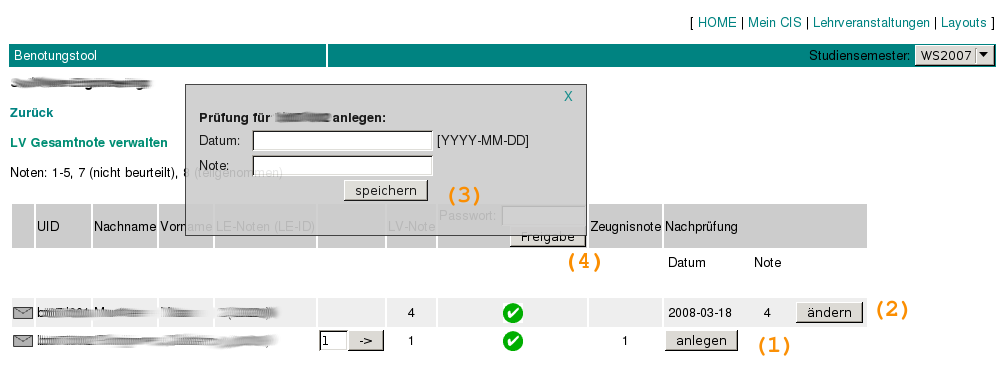
\includegraphics[width=1.0\textwidth]{benotungstool_benotung_lv_nachpruefung.png}
\end{center}
\caption{Final Grade for a Course - Resit}\label{benotung_lv_nachpruefung_quick}
\end{figure}

Click on the respective button to create or edit a resit. Enter the date and grade in the window (3) that appears and then accept the entries by clicking on the "Save" button.

\begin{itemize}
    \item When entering the date, please use the following format: YYYY-MM-DD
    \item Valid grades are once again 1-5, 7 (not graded), 8 (particiapted) and in addition 9 (not yet entered). If you leave the field for the grade blank, then this is interpreted as 9.
    \item After entering a new grade, please do not forget to approve it again by clicking on the the "Approve" button (4).
\end{itemize}
